\section{Durchführung} \label{sec:durchführung}

\subsection{Messung des Bauteile} \label{sec:bauteile}

    Zu Beginn des Versuchs werden ein runder und ein eckiger Stab ausgemessen.
    Es werden die Länge, der Durchmesser und die Seitenlängen der Stäbe jeweils fünfmal mit
    einer Schieblehre beziehungsweise einem Maßband gemessen.

\subsection{Schematischer Aufbau}

\begin{figure}
  \centering
  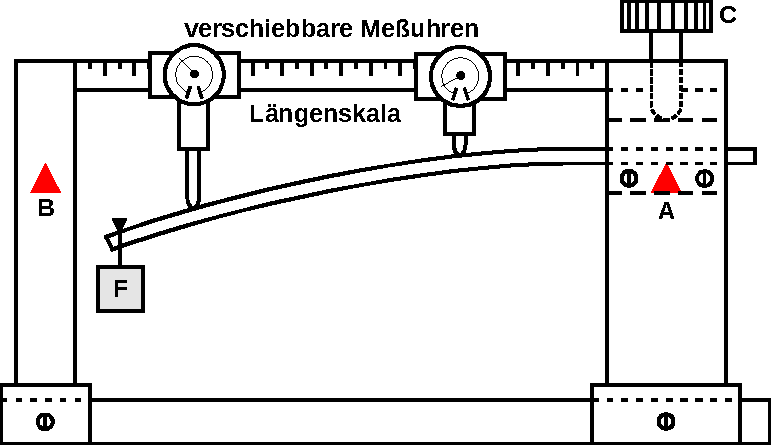
\includegraphics[width=\textwidth]{content/img/Abb_6.pdf}
  \caption{Schematischer Aufbau der Messsapparatur. \cite{img_aufbau}}
  \label{fig:aufbau}
\end{figure}

Dargestellt ist der schematische Aufbau der benutzten Messapparatur.
Diese rigide Konstruktion besitzt zwei Auflagepunkte \textbf{A} und \textbf{B},
wobei \textbf{B} nur für die beidseitige Einspannung benutzt wird,
und einer zum Fixieren benutzten Schraube \textbf{C}.
Abhängig von der Form des zu vermessenden Stabes können verschiedene Platten in \textbf{A} eingelegt werden.
Zwei verschiebbare Messuhren sind auf einer Längenskala angebracht, die die Distanz von \textbf{A} nach \textbf{B} in Millimetern angibt. Die Messuhren verfügen beide über eine Mikrometer-Skala.

\subsection{Einseitige Einspannung}

    Zuerst wird der runde Stab wie in \autoref{fig:aufbau} gezeigt in die Messapparatur eingespannt.
    Eine der verschiebbaren Messuhren wird an den Anfang der Messskala geschoben, während die andere
    nicht verwendet wird.
    Anschließend wird ein Gewicht gewählt, sodass die maximale Auslenkung des Stabes zwischen \SI{3}{\milli\meter} und \SI{7}{\milli\meter} liegt.
    Das Gewicht wird mit einer elektronischen Waage fünfmal gemessen.
    Um nun die Durchbiegung des Stabes zu messen, wird die Messuhr die Skala entlang geschoben und in
    regelmäßigen Abständen wird zuerst die Auslenkung $D_0(x)$ des runden Stabes ohne angehängtes Gewicht
    und dann mit angehängtem Gewicht $D_\text{M}$ abgelesen.
    Es werden 20 Messungen durchgeführt.

    Die Messung für den eckigen Stab erfolgt analog.

\subsection{Beidseitige Einspannung}

    Diese Messung wird nur für den runden Stab durchgeführt.
    Der Stab wird in der Messapparatur an den Enden an den Punkten A und B (siehe \autoref{fig:aufbau})
    befestigt.
    Es wird ein Gewicht bestimmt, mit dem die maximale Auslenkung des Stabes zwischen \SI{3}{\milli\meter} und \SI{7}{\milli\meter} liegt
    und mit einer elektronischen Waage fünfmal ausgemessen.
    Eine Messuhr wird an den Anfang der Messskala geschoben, die andere an das Ende.
    Um die Durchbiegung zu messen, wird die Messuhr die Skala entlang geschoben und in regelmäßigen Abständen
    werden im Wechsel eine Nullmessung und eine Messung mit angehängtem Gewicht durchgeführt.
    Es werden 16 Messungen durchgeführt.
